\section{Resultados}

\begin{figure}[h]
\centering
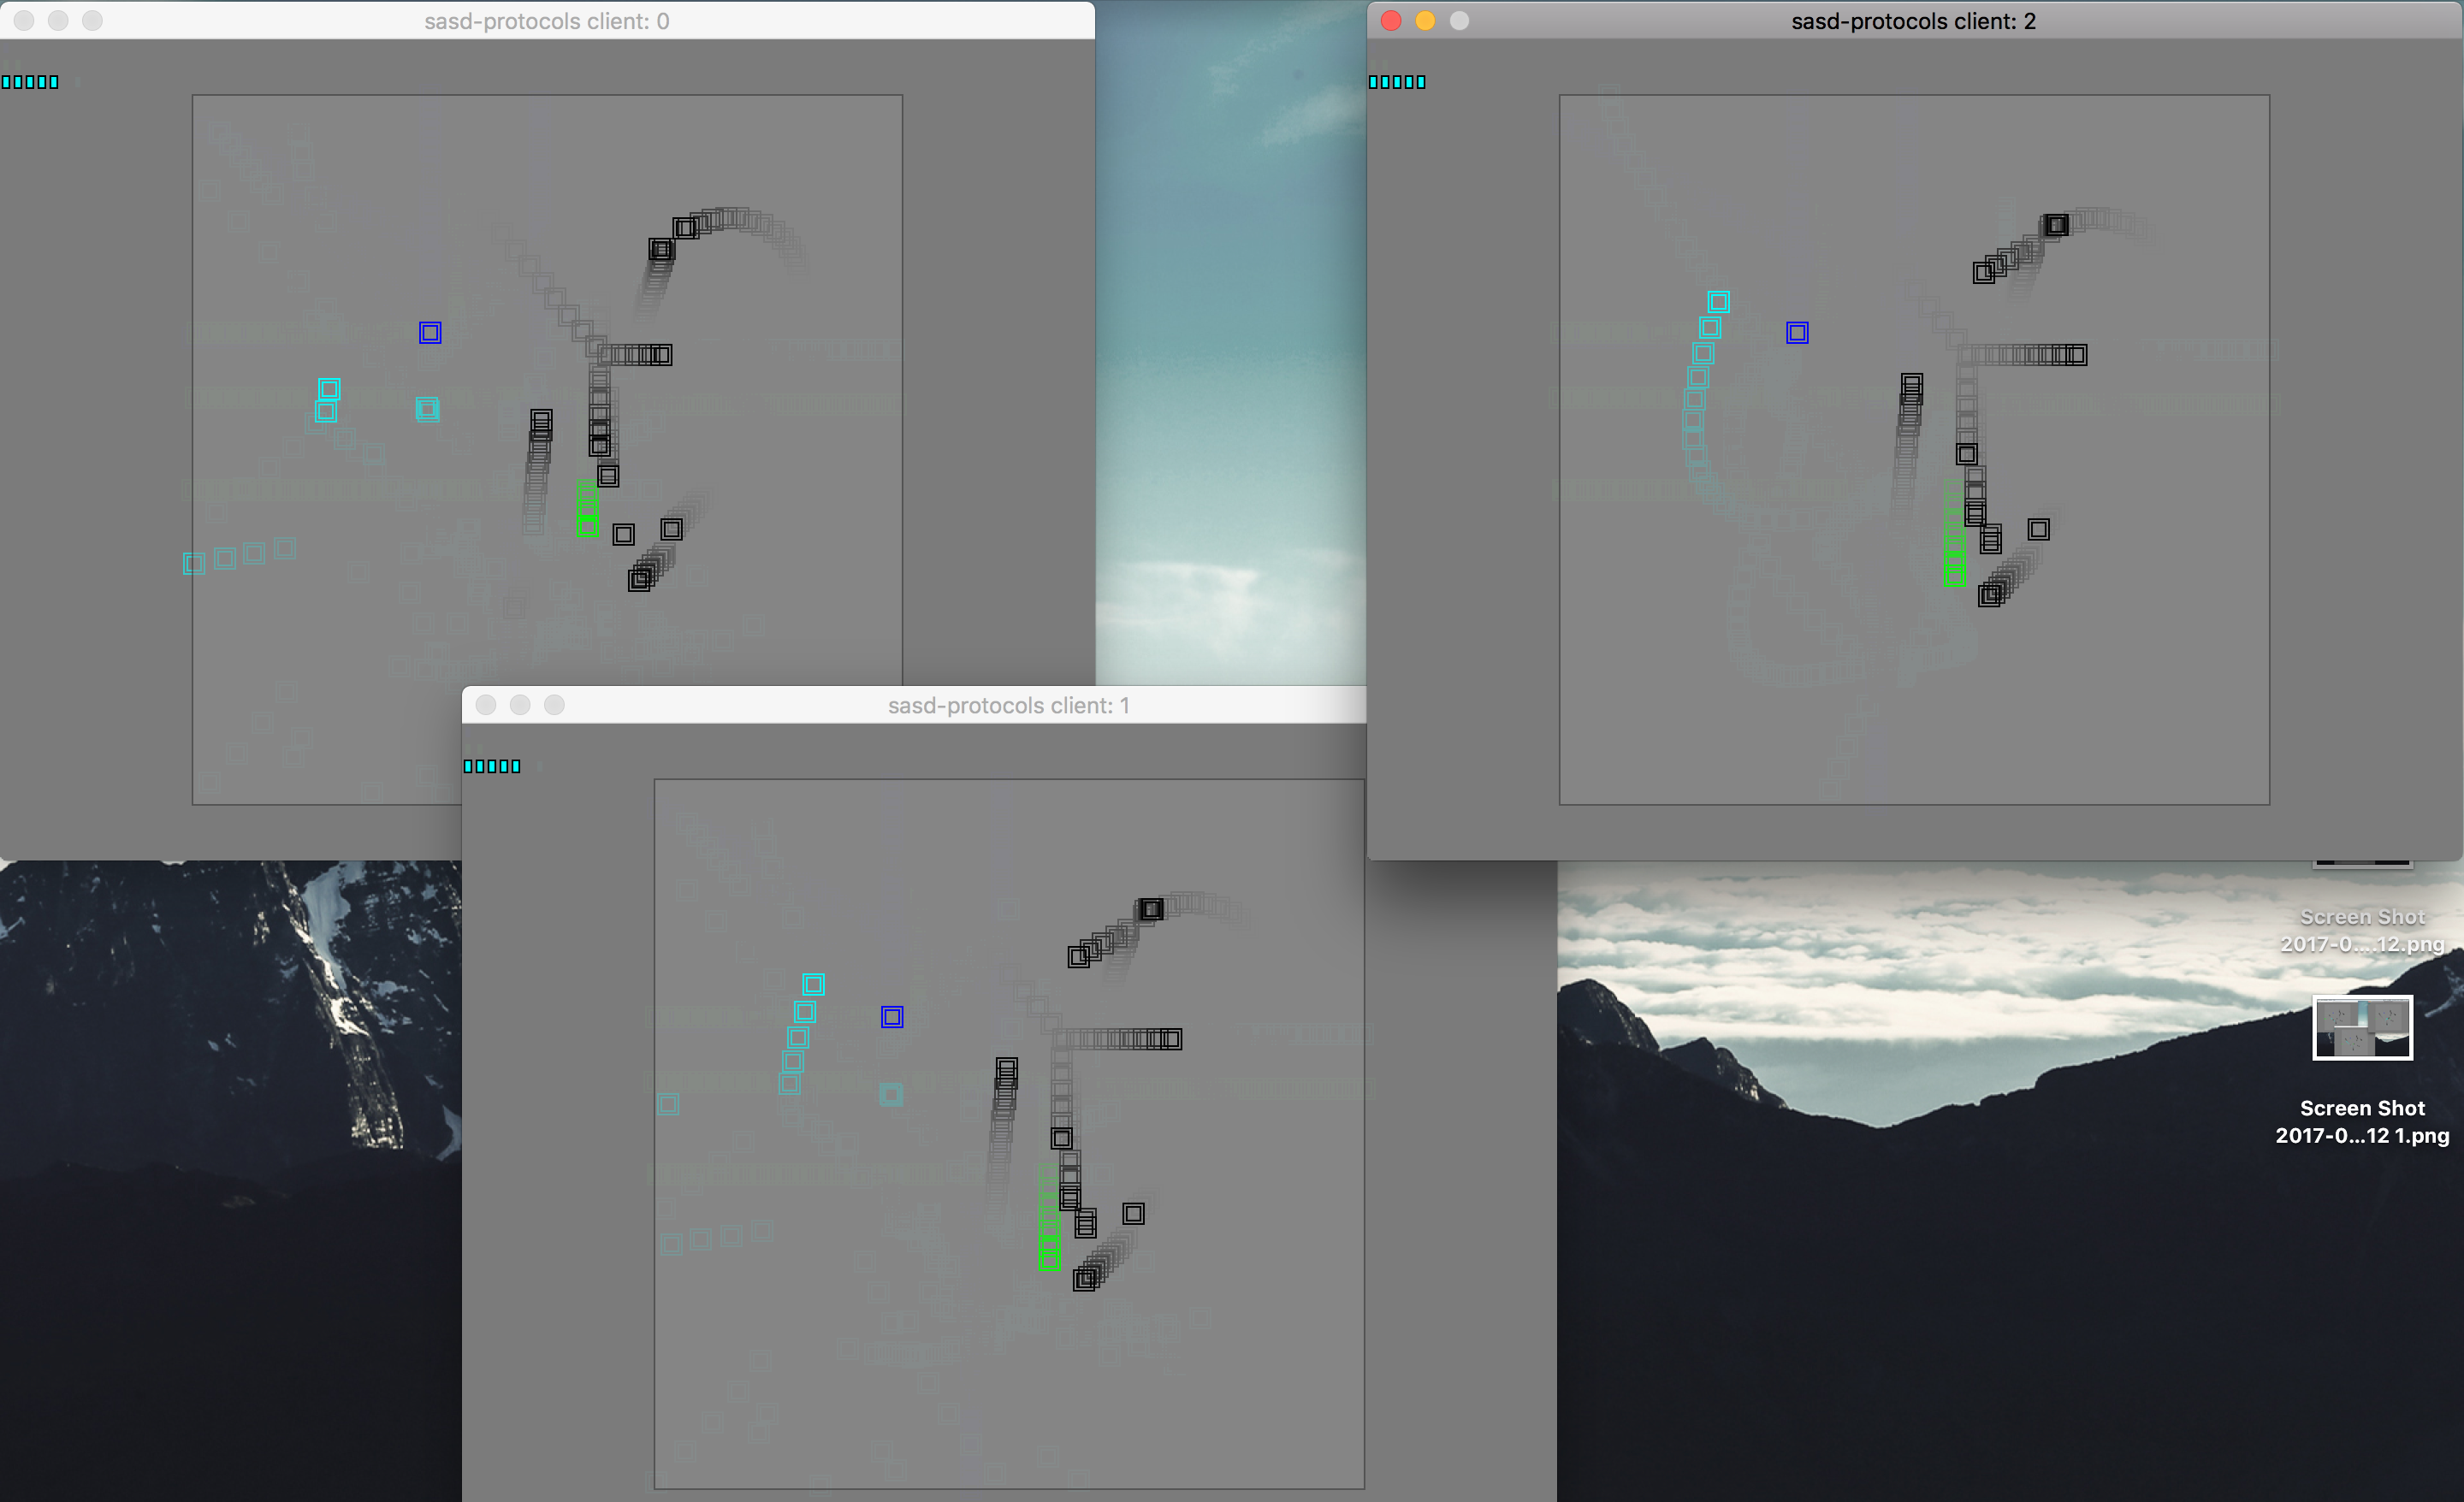
\includegraphics[width=0.8\textwidth]{run}
\caption{\label{fig:execution} \small Ejecución de varios clientes conectados corriendo en una misma máquina con el protocolo \emph{Timewarp} implementado en el \emph{framework}.} Se simuló una gran latencia entre los clientes, se puede ver que el cliente $2$ (color celeste) se movió hacia arriba y los otros tuvieron que aplicar \emph{rollbacks}, lo que se vio como un salto.
\end{figure}


% Identificar cualitativamente los resultados del retraso de la red en cada uno de los métodos.
